% Completa los datos convenientemente en las zonas marcadas con TODO

\documentclass{beamer}
%PARA VISUALIZAR PRESENTACIONN CON NOTAS USAR VISUALIZADOR "pdfpc":
%Para ver las notas, el cronometro y siguente diapo:
% pdfpc --notes=right slides.pdf
% "tecla p": para pausar el cronometro
\mode<presentation> {
  \usetheme{CambridgeUS}
  \usecolortheme{crane} % color naranja
}

\definecolor{myblue}{RGB}{250,181,235}
\definecolor{myblack}{RGB}{84,41,84}
\setbeamercolor*{structure}{bg=myblue!20,fg=myblue}

\setbeamercolor*{palette primary}{use=structure,fg=white,bg=structure.fg}
\setbeamercolor*{palette secondary}{use=structure,fg=white,bg=structure.fg!75} %fondo de abajo en medio
\setbeamercolor*{palette tertiary}{use=structure,fg=white,bg=black} %fondo de la izquierda
%\setbeamercolor*{palette quaternary}{fg=white,bg=black}

%\setbeamercolor{section in toc}{fg=black,bg=white}
\setbeamercolor{alerted text}{use=structure,fg=structure.fg!50!black!80!black}

%\setbeamercolor{titlelike}{parent=palette primary,fg=structure.fg!50!black}
\setbeamercolor{frametitle}{bg=myblue!85,fg=white} %Barra de titulo (contenidos, etc)

\setbeamercolor*{titlelike}{parent=palette primary}


%\definecolor{myblue}{RGB}{250,181,235}
%\setbeamercolor*{structure}{bg=myblue!20,fg=myblue}

%\setbeamercolor*{palette primary}{use=structure,fg=white,bg=structure.fg}
%\setbeamercolor*{palette secondary}{use=structure,fg=white,bg=structure.fg!75}


%\setbeamercolor{titlelike}{parent=structure,bg=myblue,fg=structure.fg!50!black}
%\setbeamercolor{frametitle}{bg=myblue!85,fg=white}
%\setbeamercolor{section in toc}{fg=black,bg=white}

%\setbeamercolor{titlelike}{parent=structure,bg=myblue} % Cambia el color de la caja del título de la página inicial

\setbeamertemplate{navigation symbols}{} % ocultar iconos de navegación
\setbeamerfont{subsection in toc}{size=\small} % reducir tamaño en TOC
\setbeamerfont{date}{size=\tiny}
\usepackage[spanish]{babel}
\usepackage[utf8]{inputenc}
\usepackage{graphicx}
\usepackage{booktabs}
\usepackage{hyperref}
\usepackage{multicol}
\usepackage{pgfpages}
\usepackage{listings}
\usepackage{multimedia}
\usepackage[export]{adjustbox}
\usepackage{outlines} % Para poner bullets tabulados (\1 \2 \3 ...) y no items

\usepackage{array,tabularx} % para tabular leyenda de ecuaciones
\newenvironment{conditions*} % entorno de "leyenda de ecuación"
  {\par\vspace{\abovedisplayskip}\noindent
   \tabularx{\columnwidth}{>{$}l<{$} @{\ : } >{\raggedright\arraybackslash}X}}
  {\endtabularx\par\vspace{\belowdisplayskip}}
  
% USO DE NOTAS
\setbeameroption{hide notes} % Para mostrar u ocultar (hide/show)
%\setbeameroption{show only notes} % Mostrar solo las notas
%\setbeameroption{show notes on second screen=right} % Mostrar notas en otra pantalla
\setbeamertemplate{note page}{ % asi solo muestro el texto de las notas
  \insertnote%
}

%========= TODO: datos internos del documento
\hypersetup{
	pdftitle={Defensa de trabajo de fin de grado de Isabel Cebollada Gracia},
	pdfauthor={Isabel Cebollada Gracia},
	pdfsubject={Sistema de monitorización para el control y estudio del bienestar de animales de laboratorio mediante una infraestructura de bajo coste},
	pdfkeywords={raspberry, inteligencia artificial, machine learning, deep learning, visión artificial},
	pdfproducer={pdfLaTeX},
  colorlinks=true,
  linkcolor=blue
}
%=========

%========= TODO: diapositiva de portada
\title[Sistema de monitorización]{Sistema de monitorización para el control y estudio del bienestar de animales de laboratorio mediante una infraestructura de bajo coste} % El título reducido aparece en la parte inferior de todas las diapositivas
                                         % El título completo aparece solo en la diapositiva de portada
\author[Isabel Cebollada Gracia]{Isabel Cebollada Gracia}
\institute[URJC]
{
\textit{\href{mailto:i.cebollada.2018@alumnos.urjc.es}{\color{blue}{\underline{i.cebollada.2018@alumnos.urjc.es}}}}\\
\vspace{0.5cm}

\includegraphics[width=3cm]{figs/logo-urjc}\\
\vspace{1cm}
Trabajo fin de grado
}
\date{27 de Julio de 2022}
%=========

%========= COMIENZO DEL DOCUMENTO
\begin{document}

%========= Portada inicial con notas
\begin{frame}[plain] % plain: quita header y footer
\large{\titlepage}
\note[item]{En esta presentación voy a hablar sobre...}
\note[item]{En primer lugar...}
\end{frame}

%========= Licencia
\begin{frame}
% Este diseño se corresponde con la licencia CC-BY-NC-SA.
% Por supuesto, puedes poner la licencia que mejor se adapte al propósito de tu trabajo.
% Recuerda que, si no se especifica ninguna licencia, esta -como cualquier creación artística- pasaría a estar licenciada con todos los derechos reservados (copyright).

\cleardoublepage

\begin{figure}
 \ \ \ \ 
\includegraphics[width=0.25\linewidth]{figs/by-nc-sa.png}
 \label{fig:cc} 
 \end{figure}

\

\

\

\noindent
Este trabajo se distribuye bajo los términos de la licencia internacional \href{http://creativecommons.org/licenses/by-nc-sa/4.0/}{CC BY-NC-SA International License} (Creative Commons AttributionNonCommercial-ShareAlike 4.0). Usted es libre de \textit{(a) compartir}: copiar y redistribuir el material en cualquier medio o formato; y \textit{(b) adaptar}: remezclar, transformar y crear a partir del material. El licenciador no puede revocar estas libertades mientras cumpla con los términos de la licencia:

\begin{itemize}
\item \textit{Atribución}. Usted debe dar crédito de manera adecuada, brindar un enlace a la licencia, e indicar si se han realizado cambios. Puede hacerlo en cualquier forma razonable, pero no de forma tal que sugiera que usted o su uso tienen el apoyo de la licenciante.
\item \textit{No comercial}. Usted no puede hacer uso del material con propósitos comerciales.
\item \textit{Compartir igual}. Si remezcla, transforma o crea a partir del material, debe distribuir su contribución bajo la la misma licencia del original.
\end{itemize}

\begin{flushright}
		\vspace{7.0 cm}
		\emph{Documento de} \textbf{Isabel Cebollada}. % TODO: pon aquí tu nombre cuando hagas el documento
\end{flushright}


\end{frame}

%========= Índice o tabla de contenidos (TOC)
\begin{frame}
\frametitle{Contenidos}
%\begin{multicols}{2} % si tengo muchas secciones, lo parte en dos columnas
  \tableofcontents[hideallsubsections] % no muestra subsecciones
%\end{multicols}
\note[item]{La presentaci\'on esta dividida en cuatro partes.}
\end{frame}

%========= Diapositiva "vacía" de comienzo de sección:
\section*{}
\begin{frame}{}
  \centering \Huge
  \emph{Introducción}
\note[item]{Comencemos con la introducción a la robótica.}
\end{frame}

\section{Introducción}
\subsection{Contexto general}
%========= Diapositiva con imágenes:
\begin{frame}
\frametitle{Introducción a la robótica}
¿Qué es la robótica?
\begin{itemize}
\item Campo de investigación muy importante que continua en desarrollo.
\item Objetivo: Realizar trabajos \textcolor{magenta}{aburridos}, \textcolor{magenta}{sucios} o \textcolor{magenta}{pesados} para el humano.
\end{itemize}
\note[item]{La robótica es un campo de investigación muy importante en la actualidad que continua en desarrollo, cuyo objetivo es realizar trabajos que resultan pesados, aburridos o sucios para el ser humano.}
\end{frame}

\begin{frame}
\frametitle{Definición de robot}
¿Qué es un robot?
\begin{figure}
\centering
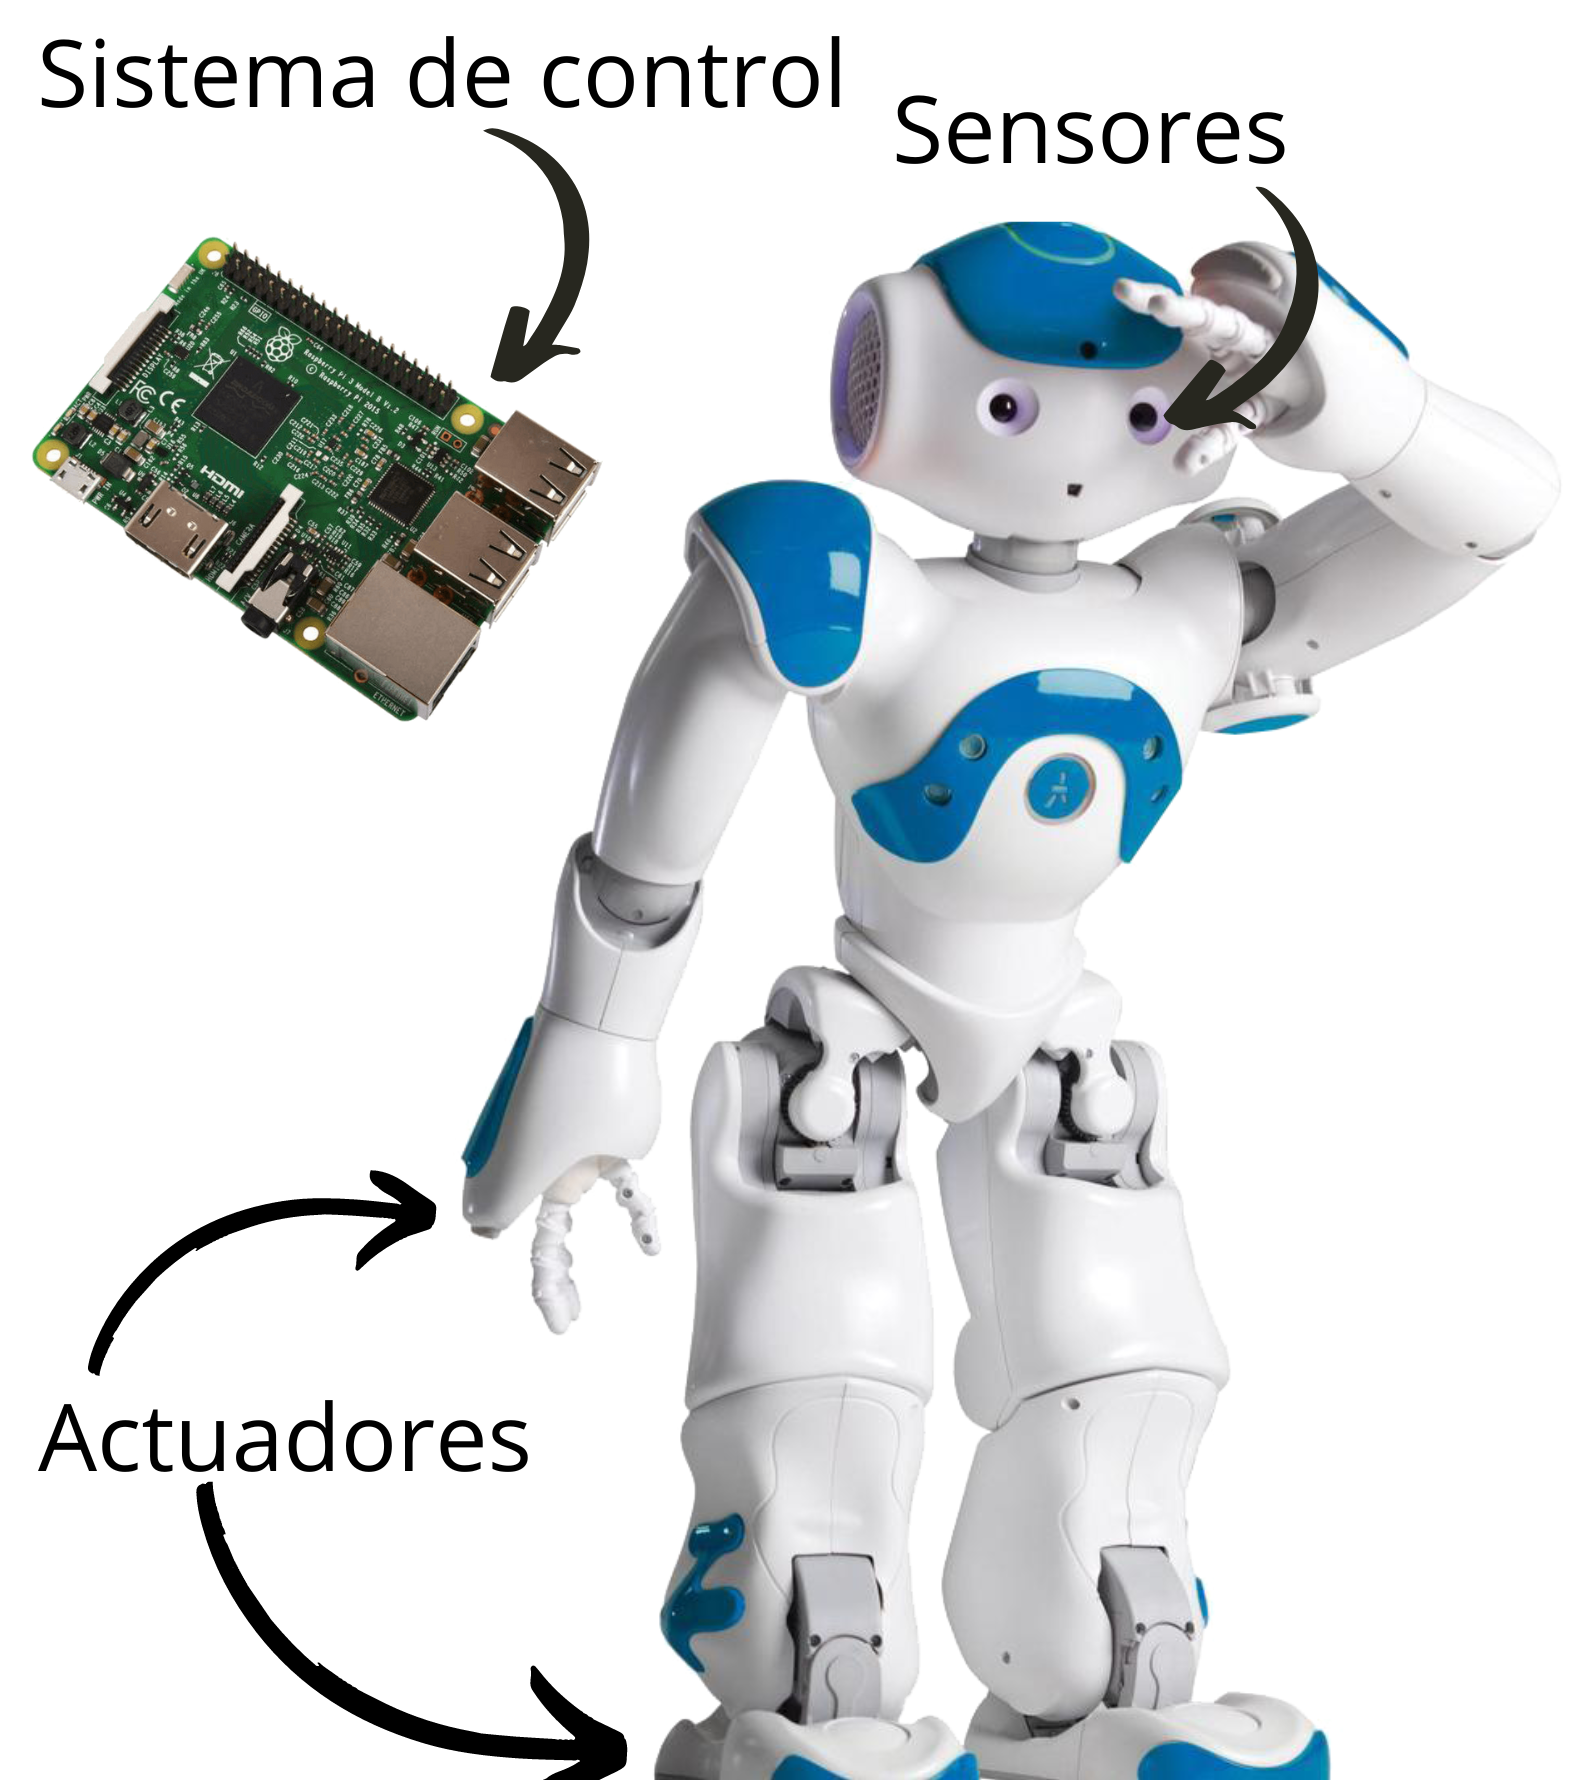
\includegraphics[width=6cm]{figs/robot}
\end{figure}
\note[item]{A lo largo de los años el concepto de robótica ha ido variando, así como la definición de robot. Actualmente, se entiende por robot a cualquier dispositivo dotado por sensores, actuadores y un sistema de control.}
\end{frame}

\begin{frame}
\frametitle{Algunos tipos de sensores}
\begin{figure}
\centering
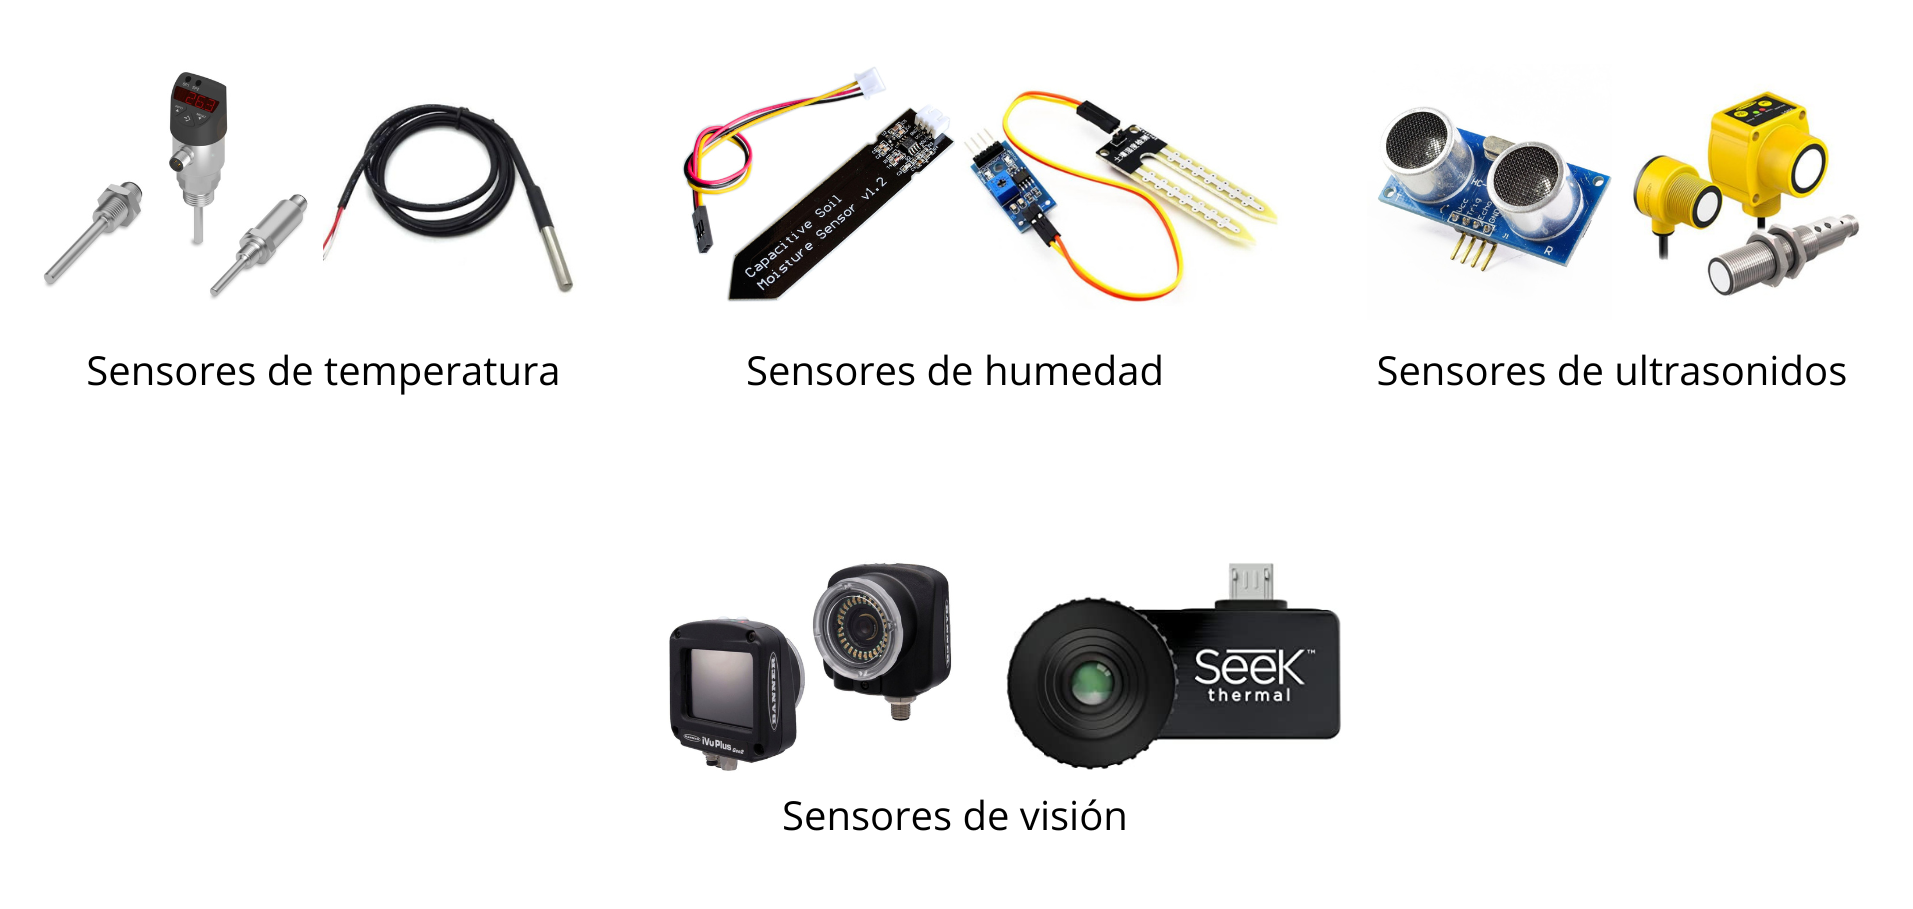
\includegraphics[width=12cm]{figs/sensores}
\end{figure}
\note[item]{Existen distintos tipos de sensores que dotan de distintas cualidades. Entre ellos, uno de los más importantes es el sensor de visión, que requiere un proceso arduo para extraer información útil en tiempo real. Para el procesamiento de la información obtenida del sensor de visión, es necesario aplicar un algoritmo de IA.}
\end{frame}

\begin{frame}
\frametitle{Inteligencia Artificial}
\begin{figure}
\centering
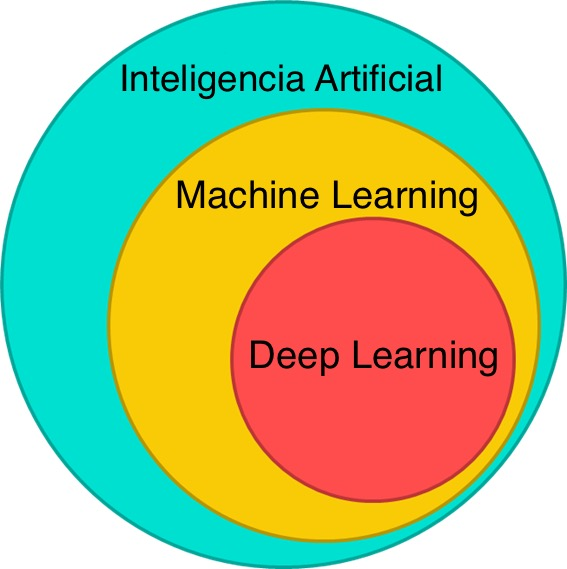
\includegraphics[width=6cm]{figs/ia}
\end{figure}
\note[item]{La inteligencia artificial consiste en replicar los mecanismos del cerebro mediante algoritmos. Uno de los algoritmos más usados es el ML, preprogramados por un humano y que tratan de descubrir patrones que les hacen aprender. Los algoritmos más usados en visión artificial pertenecen a un subcampo del ML denominado DL, donde el autómata aprende por si mismo sin intervención humana, simulando el cerebro con unidades equivalentes a las neuronas.}
\end{frame}

\begin{frame}
\frametitle{Sistemas multisensoriales}
\begin{figure}
\centering
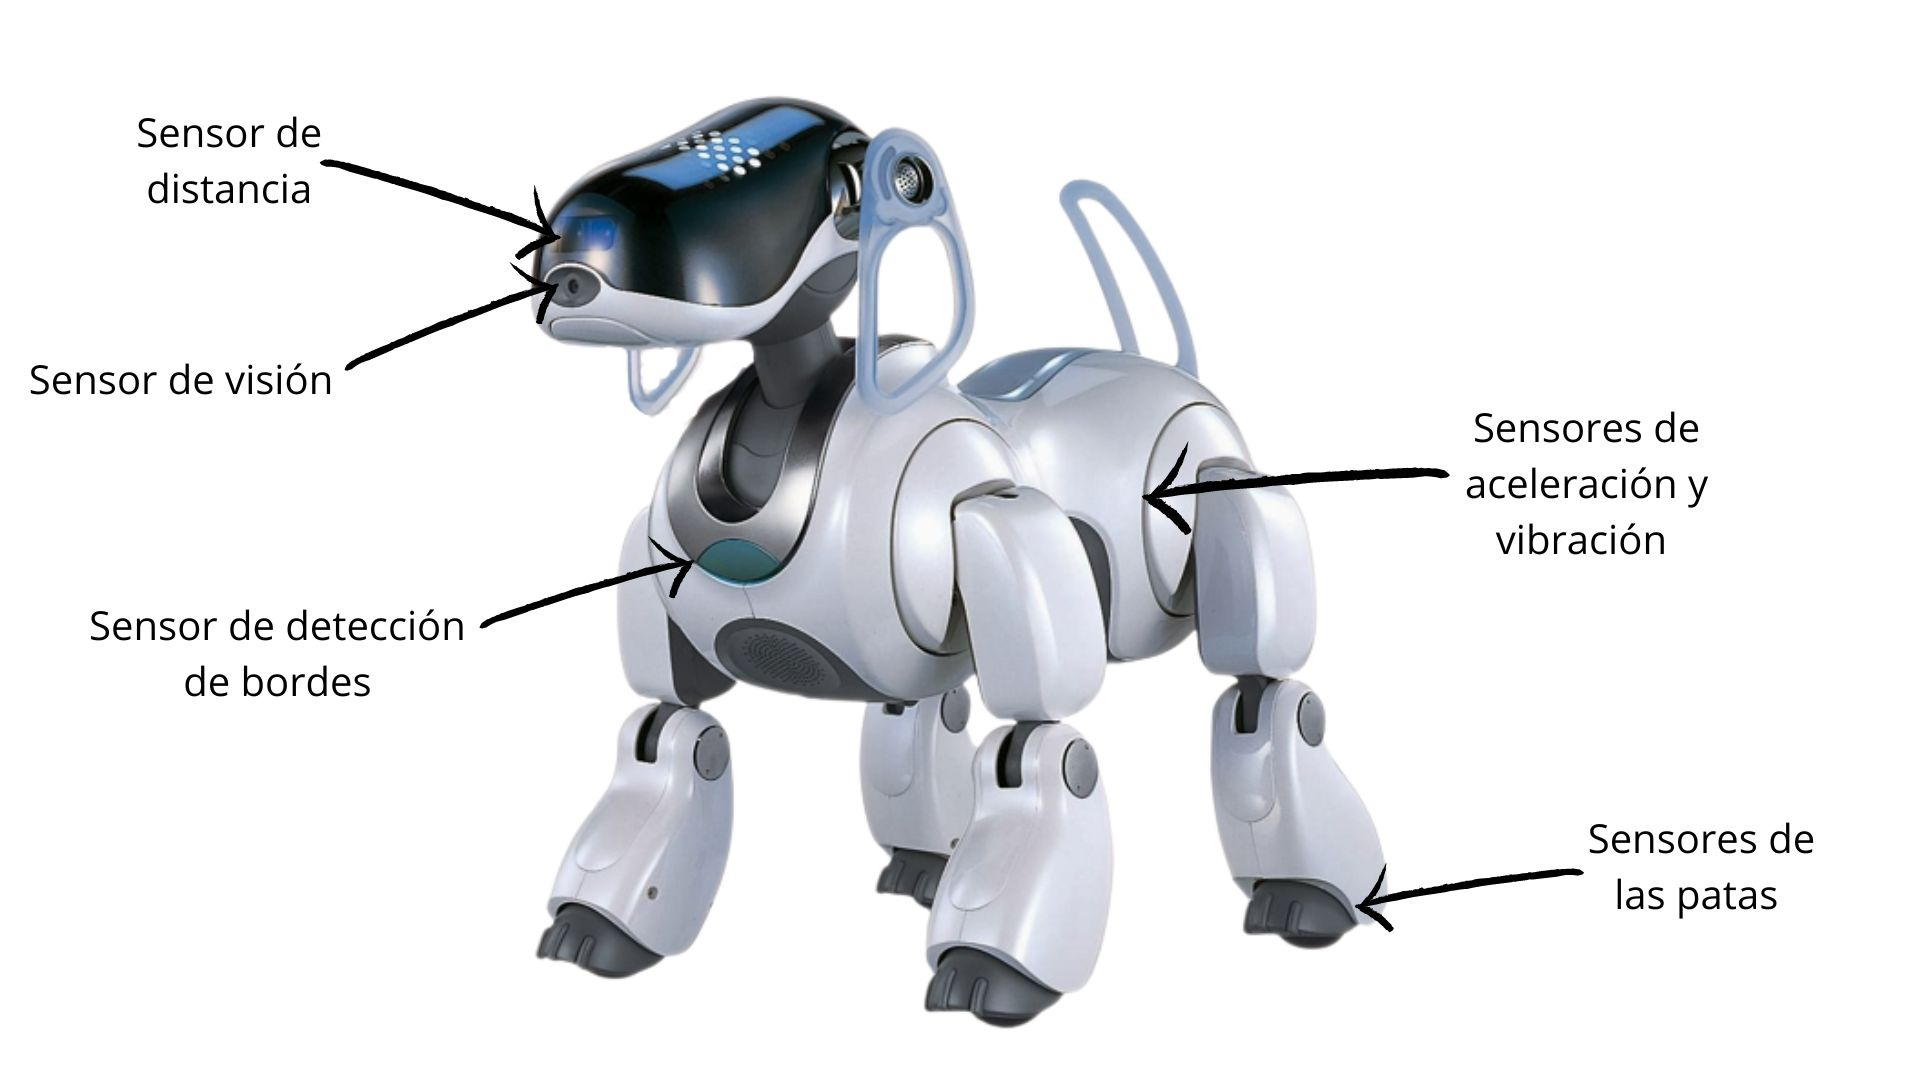
\includegraphics[width=12cm]{figs/multisensorial}
\end{figure}
\note[item]{Además de utilizar sensores de visión, si a un robot se le incorporan diferentes tipos de sensores, este obtendrá mucha más información, por lo que podrá ser más preciso y simular a un humano mejor. Este trabajo se enmarca en el contexto de los sistemas multisensoriales, concretamente en los sistemas multisensoriales destinados al bienestar animal y al análisis de comportamiento.}
\end{frame}

%========= Diapositiva con ítems resaltados con colores:
\begin{frame}
\frametitle{Introducción a la Robótica}
\begin{itemize}
\item La \textcolor{red}{tecnología} está cada vez más presente en la vida cotidiana.
\item Los robots de servicio aparecen en el \textcolor{blue}{mercado}.
\item La \textcolor{red}{domótica} presenta cada vez más aplicaciones domésticas.
\end{itemize}
\end{frame}

\subsection{Contexto específico}
%========= Diapositiva con bloques:
\begin{frame}
\frametitle{Precedentes de la robótica}
\begin{block}{Primera revolución industrial de 1800}
Productos fabricados por \textcolor{blue}{máquinas}. La \textcolor{red}{máquina de vapor} fue clave.
\end{block}
\end{frame}

%========= Diapositiva con bullets en diferentes niveles (outline):
\section{Principios de transducción}
\subsection{Principio de transducción piezoresistivo}
\begin{frame}
\frametitle{Conceptos}
\begin{outline}
\1 Piezoresistividad: relación entre resistencia eléctrica y deformación.
\2 Material piezoresistivo: (1) material en reposo (átomos en equilibrio).
\3 (2) Si sufre deformación, movimiento átomos, modifican su resistividad.
\2 Resistencia vs. resistividad de un material.
\3 Resistencia: depende del volumen del material a tratar.
\3 Resistividad: caract. intrínseca relacionada con colocación de átomos.
\end{outline}
\end{frame}

\section*{}
\begin{frame}{}
  \centering \Huge
  \emph{Objetivos}
\note[item]{Pasemos ahora a comentar los objetivos que nos hemos con este trabajo.}
\end{frame}

\section{Objetivos}
\begin{frame}
\begin{enumerate}
\item Crear una herramienta multiplataforma.
\item Sin necesidad de instalación.
\item Toda ejecución vía web.
\end{enumerate}
\end{frame}

\section*{}
\begin{frame}{}
  \centering \Huge
  \emph{Diseño}
\note[item]{Una vez descritos los objetivos, veamos qué hemos hecho para alcanzarlos.}
\end{frame}

\section{Diseño}
%========= Diapositiva con matemáticas:
\subsection{Matemáticas empleadas}
\begin{frame}
\frametitle{Matrices de la cámara}
\begin{itemize}
\item Se usa una matriz $RT (4x4)$ en lugar de $R$ y $T$.
\item La matriz $RT$ rota $\theta$ grados en los ejes $X$, $Y$ y $Z$:
\end{itemize}
\begin{equation}
	\begin{bmatrix}
	1 & 0 & 0 & X \\
	0 & cos(\theta) & sin(\theta) &	Y \\
	0 & -sin(\theta)& cos(\theta) & Z \\
	0 & 0 & 0 & 1 
	\end{bmatrix}
\end{equation}
\end{frame}

%========= Diapositiva con matemáticas y leyenda (conditions*):
\begin{frame}
\frametitle{Resistencia de un material}
\begin{outline}
\1 Si material piezoresistivo se deforma, cambia su resistencia eléctrica.
\begin{equation}
R=\rho\frac{l}{A}
\end{equation}
donde:
\begin{conditions*}
R & resistencia del material $[\Omega]$\\
\rho & resistividad $[\Omega-m]$\\
l & longitud $[m]$\\
A & área de sección transversal $[m^2]$
\end{conditions*}
\1 El cambio de resistencia se obtiene a partir de:
\begin{equation}
\frac{\Delta R}{R}=\frac{\Delta\rho}{\rho}=\frac{\Delta A}{A}=\frac{\Delta l}{l}
\end{equation}
\1 Otra forma de medir el efecto piezoresistivo: el factor de deformación.
\begin{equation}
GF(\textit{Gauge Factor})=\frac{\frac{\Delta R}{R}}{\varepsilon}=\frac{\frac{\Delta R}{R}}{\frac{\Delta l}{l}}
\end{equation}
\end{outline}
\end{frame}

%========= Diapositiva con códigos:
\subsection{Algoritmo principal}
\begin{frame}[fragile]
\frametitle{Algoritmo de visión}
\begin{lstlisting}
cvCvtColor (&image, IplTmp1, CV_RGB2GRAY);//to Gray
cvNormalize(IplTmp1, IplTmp1, 0, 255, CV_MINMAX);
cvSmooth(IplTmp1,IplTmp2,CV_BLUR,3,3);//Avrg filter
cvLaplace(IplTmp2, IplLaplace, 3);//Laplace
cvConvertScale(IplLaplace,IplTmp1);
cvThreshold(IplTmp1,IplTmp2,Thress,255,CV_THRESH_BIN);
\end{lstlisting}
\end{frame}

\section*{}
\begin{frame}{}
  \centering \Huge
  \emph{Conclusiones}
\note[item]{Para acabar esta presentación, vamos a repasar lo hecho, unas breves conclusiones y las líneas futuras.}
\end{frame}

\section{Conclusiones}
\begin{frame}
\begin{block}{Objetivos cumplidos}
\begin{itemize}
\item Herramienta multiplataforma: soporta Linux, Windows, MacOS.
\item Intuitiva para el usuario final: no se necesita instalar nada.
\item Solo se necesita un navegador web.
\end{itemize}
\end{block}

\begin{block}{Líneas futuras}
\begin{itemize}
\item Permitir el uso de otras herramientas.
\item Ampliar los botones disponibles en el interfaz.
\end{itemize}
\end{block}
\end{frame}

\begin{frame}[plain]
\large{\titlepage}
\note[item]{Y hasta aquí mi exposición.}
\note[item]{Quedo a disposición del tribunal...}
\end{frame}

\end{document}
